%  LaTeX support: latex@mdpi.com 
%  In case you need support, please attach all files that are necessary for compiling as well as the log file, and specify the details of your LaTeX setup (which operating system and LaTeX version / tools you are using).

% You need to save the "mdpi.cls" and "mdpi.bst" files into the same folder as this template file.
% Add inline option to enumitem package
\PassOptionsToPackage{inline}{enumitem}
%=================================================================
\documentclass[symmetry,article,submit,moreauthors,pdftex,10pt,a4paper]{Definitions/mdpi} 
\usepackage{threeparttable}
\usepackage{array}
\newcolumntype{L}[1]{>{\raggedright\let\newline\\\arraybackslash\hspace{0pt}}m{#1}}
\newcolumntype{C}[1]{>{\centering\let\newline\\\arraybackslash\hspace{0pt}}m{#1}}
\newcolumntype{R}[1]{>{\raggedleft\let\newline\\\arraybackslash\hspace{0pt}}m{#1}}
%abbr: eg, ie, etc, et al,
\usepackage{xspace}
\newcommand*{\eg}{e.g.\@\xspace}
\newcommand*{\ie}{i.e.\@\xspace}
\makeatletter
\newcommand*{\etc}{%
    \@ifnextchar{.}%
        {etc}%
        {etc.\@\xspace}%
}
\newcommand*{\etal}{%
    \@ifnextchar{.}%
        {et al}%
        {et al.\@\xspace}%
}

% If you would like to post an early version of this manuscript as a preprint, you may use preprint as the journal and change 'submit' to 'accept'. The document class line would be, e.g. \documentclass[preprints,article,accept,moreauthors,pdftex,10pt,a4paper]{mdpi}. This is especially recommended for submission to arXiv, where line numbers should be removed before posting. For preprints.org, the editorial staff will make this change immediately prior to posting.

%
%--------------------
% Class Options:
%--------------------
% journal
%----------
% Choose between the following MDPI journals:
% acoustics, actuators, addictions, admsci, aerospace, agriculture, agronomy, algorithms, animals, antibiotics, antibodies, antioxidants, applsci, arts, asi, atmosphere, atoms, axioms, batteries, bdcc, behavsci, beverages, bioengineering, biology, biomedicines, biomimetics, biomolecules, biosensors, brainsci, buildings, carbon, cancers, catalysts, cells, ceramics, challenges, chemengineering, chemosensors, children, cleantechnol, climate, clockssleep, cmd, coatings, colloids, computation, computers, condensedmatter, cosmetics, cryptography, crystals, cybersecurity, data, dentistry, designs, diagnostics, dairy, diseases, diversity, drones, econometrics, economies, education, electrochem, electrochemistry, electronics, energies, entropy, environments, epigenomes, est, fermentation, fibers, fire, fishes, fluids, foods, forecasting, forests, fractalfract, futureinternet, galaxies, games, gastrointestdisord, gels, genealogy, genes, geohazards, geosciences, geriatrics, hazardousmatters, healthcare, heritage, highthroughput, horticulturae, humanities, hydrology, informatics, information, infrastructures, inorganics, insects, instruments, ijerph, ijfs, ijms, ijgi, ijtpp, inventions, j, jcdd, jcm, jcs, jdb, jfb, jfmk, jimaging, jof, jintelligence, jlpea, jmmp, jmse, jpm, jrfm, jsan, land, languages, laws, life, literature, logistics, lubricants, machines, magnetochemistry, make, marinedrugs, materials, mathematics, mca, medsci, medicina, medicines, membranes, metabolites, metals, microarrays, micromachines, microorganisms, minerals, modelling, molbank, molecules, mps, mti, nanomaterials, ncrna, neonatalscreening, neuroglia, nitrogen, nutrients, ohbm, particles, pathogens, pharmaceuticals, pharmaceutics, pharmacy, philosophies, photonics, plants, plasma, polymers, polysaccharides, proceedings, processes, proteomes, publications, quaternary, qubs, reactions, recycling, religions, remotesensing, reports, resources, risks, robotics, safety, sci, scipharm, sensors, separations, sexes, sinusitis, smartcities, socsci, societies, soilsystems, sports, standards, stats, surfaces, surgeries, sustainability, symmetry, systems, technologies, toxics, toxins, tropicalmed, universe, urbansci, vaccines, vehicles, vetsci, vibration, viruses, vision, water, wem, wevj
%---------
% article
%---------
% The default type of manuscript is article, but can be replaced by: 
% abstract, addendum, article, benchmark, book, bookreview, briefreport, casereport, changes, comment, commentary, communication, conceptpaper, correction, conferenceproceedings, conferencereport, expressionofconcern, meetingreport, creative, datadescriptor, discussion, editorial, essay, erratum, hypothesis, interestingimages, letter, meetingreport, newbookreceived, opinion, obituary, projectreport, reply, reprint, retraction, review, perspective, protocol, shortnote, supfile, technicalnote, viewpoint
% supfile = supplementary materials
% protocol: If you are preparing a "Protocol" paper, please refer to http://www.mdpi.com/journal/mps/instructions for details on its expected structure and content.
%----------
% submit
%----------
% The class option "submit" will be changed to "accept" by the Editorial Office when the paper is accepted. This will only make changes to the frontpage (e.g. the logo of the journal will get visible), the headings, and the copyright information. Also, line numbering will be removed. Journal info and pagination for accepted papers will also be assigned by the Editorial Office.
%------------------
% moreauthors
%------------------
% If there is only one author the class option oneauthor should be used. Otherwise use the class option moreauthors.
%---------
% pdftex
%---------
% The option pdftex is for use with pdfLaTeX. If eps figures are used, remove the option pdftex and use LaTeX and dvi2pdf.

%=================================================================
\firstpage{1} 
\makeatletter 
\setcounter{page}{\@firstpage} 
\makeatother
\pubvolume{xx}
\issuenum{1}
\articlenumber{1}
\pubyear{2018}
\copyrightyear{2018}
\externaleditor{Academic Editor: name}
\history{Received: date; Accepted: date; Published: date}

%\updates{yes} % If there is an update available, un-comment this line
 
%------------------------------------------------------------------
% The following line should be uncommented if the LaTeX file is uploaded to arXiv.org
%\pdfoutput=1

%=================================================================
% Add packages and commands here. The following packages are loaded in our class file: fontenc, calc, indentfirst, fancyhdr, graphicx, lastpage, ifthen, lineno, float, amsmath, setspace, enumitem, mathpazo, booktabs, titlesec, etoolbox, amsthm, hyphenat, natbib, hyperref, footmisc, geometry, caption, url, mdframed, tabto, soul, multirow, microtype, tikz

%=================================================================
%% Please use the following mathematics environments: Theorem, Lemma, Corollary, Proposition, Characterization, Property, Problem, Example, ExamplesandDefinitions, Hypothesis, Remark, Definition
%% For proofs, please use the proof environment (the amsthm package is loaded by the MDPI class).

%=================================================================
% Full title of the paper (Capitalized)
\Title{Rank Correlation of Centrality Metrics in Complex Networks: An Empirical Study}

% Author Orchid ID: enter ID or remove command
\newcommand{\orcidauthorA}{0000-0002-5479-2256} % Add \orcidA{} behind the author's name
%\newcommand{\orcidauthorB}{0000-0000-000-000X} % Add \orcidB{} behind the author's name

% Authors, for the paper (add full first names)
\Author{Chengcheng Shao $^{1}$*\orcidA{}, Pengshuai Cui $^{1}$ and Xinwen Jiang $^{2,}$}

% Authors, for metadata in PDF
\AuthorNames{Chengcheng Shao, Pengshuai Cui and Xinwen Jiang}

% Affiliations / Addresses (Add [1] after \address if there is only one affiliation.)
\address{%
$^{1}$ \quad College of Computer, National University of Defense Technology, Changsha, 410073 Hunan, China\\
$^{2}$ \quad The MOE Key Laboratory of Intelligent Computing and Information Processing, Xiangtan University, 411105 Hunan, China}

% Contact information of the corresponding author
\corres{Correspondence: sccotte@gmail.com}

% Current address and/or shared authorship
% \firstnote{Current address: Affiliation 3} 
% \secondnote{These authors contributed equally to this work.}
% The commands \thirdnote{} till \eighthnote{} are available for further notes

% Simple summary
%\simplesumm{}

% Abstract (Do not insert blank lines, i.e. \\) 
\abstract{A single paragraph of about 200 words maximum. For research articles, abstracts should give a pertinent overview of the work. We strongly encourage authors to use the following style of structured abstracts, but without headings: 1) Background: Place the question addressed in a broad context and highlight the purpose of the study; 2) Methods: Describe briefly the main methods or treatments applied; 3) Results: Summarize the article's main findings; and 4) Conclusion: Indicate the main conclusions or interpretations. The abstract should be an objective representation of the article, it must not contain results which are not presented and substantiated in the main text and should not exaggerate the main conclusions.}

% Keywords
\keyword{keyword 1; keyword 2; keyword 3 (list three to ten pertinent keywords specific to the article, yet reasonably common within the subject discipline.)}

% The fields PACS, MSC, and JEL may be left empty or commented out if not applicable
%\PACS{J0101}
%\MSC{}
%\JEL{}

%%%%%%%%%%%%%%%%%%%%%%%%%%%%%%%%%%%%%%%%%%
% Only for the journal Applied Sciences:
%\featuredapplication{Authors are encouraged to provide a concise description of the specific application or a potential application of the work. This section is not mandatory.}
%%%%%%%%%%%%%%%%%%%%%%%%%%%%%%%%%%%%%%%%%%

%%%%%%%%%%%%%%%%%%%%%%%%%%%%%%%%%%%%%%%%%%
% Only for the journal Data:
%\dataset{DOI number or link to the deposited data set in cases where the data set is published or set to be published separately. If the data set is submitted and will be published as a supplement to this paper in the journal Data, this field will be filled by the editors of the journal. In this case, please make sure to submit the data set as a supplement when entering your manuscript into our manuscript editorial system.}

%\datasetlicense{license under which the data set is made available (CC0, CC-BY, CC-BY-SA, CC-BY-NC, etc.)}

%%%%%%%%%%%%%%%%%%%%%%%%%%%%%%%%%%%%%%%%%%
% Only for the journal Toxins
%\keycontribution{The breakthroughs or highlights of the manuscript. Authors can write one or two sentences to describe the most important part of the paper.}

%\setcounter{secnumdepth}{4}
%%%%%%%%%%%%%%%%%%%%%%%%%%%%%%%%%%%%%%%%%%
\begin{document}
%%%%%%%%%%%%%%%%%%%%%%%%%%%%%%%%%%%%%%%%%%
%% Only for the journal Gels: Please place the Experimental Section after the Conclusions

%%%%%%%%%%%%%%%%%%%%%%%%%%%%%%%%%%%%%%%%%%
\section{Introduction}
\label{sec:introduction}
In  study of networks, sociologist have perhaps done the longest work to establish the best traditions in both quantitative and empirical ways~\cite{newman2010networks}. The idea of centrality was, of course, first introduced by the socialist Bavelas at 1950s, who tried to characterize the human communication in small groups of people~\cite{latora2007measure}. Since then centrality has been used to investigate  adoption of innovation\cite{coleman1966medical}, influence in interorganizational networks~\cite{laumann1973new}, employment opportunities~\cite{granovetter1995getting},  power~\cite{burt1982toward}, and \etc. While numerous metrics of centrality have been proposed in above research, the definition of centrality itself is still not beyond the general descriptors such as node prominence or structural importance~\cite{borgatti2006graph}. This unclear definition of centrality leads the interpretations of centrality measure varied, including autonomy, control, risk, exposure, influence, belongingness, brokerage, independence, power and so on. To answer the question "what is centrality", Freeman~\cite{freeman1979centrality} reviewed a number of published measures and reduced them into three basic concepts with canonical formulation. These three canonical metric were degree, closeness and betweenness that are still widely used today. Borgatti provided a more comprehensive answer in network flow view\cite{borgatti2005centrality}  and graph structure perspective~\cite{borgatti2006graph}.  In network flow context, centrality is centered on the outcomes of the nodes through which the network traffic goes. The centrality of an individual node is not necessarily determined by its structure position, but the frequency that traffic flows through the node and the time it takes to get to the node. In~\cite{borgatti2005centrality}, Borgatti laid out the typology of network flows into two dimensions:  trajectory dimension (\eg geodesics, paths, trails, or
walks) and transmission dimension (\eg broadcast, serial replication, or transfer). Thus measures of centrality becomes as predictive models of appropriate network flow properties. While the network flow perspective focuses on the outcomes of centrality, the graph-theoretic perspective is centered on how centrality measures are calculated. In~\cite{borgatti2006graph}, Borgatti  proposed a unified framework for centrality measures, which distinguishes centrality measures through four basic dimensions: Walk Type( what's the type of the involved walks, \eg geodesic or edge-disjoint), Walk Property(how many and how long of the involved walks, \eg volume and length), Walk Position(how to pass through a node of the involved walks, \eg radial or medial), and Summary Type(how to summarize rows of the walk matrix, \eg sum or average).

Today, the research of network centrality falls into two main field: application of the centrality concept into new realms and enhancement of the specified centrality computing performance. In application field, as where it is introduced, the concept of centrality is first used in social networks. Besides the early investigation of influence, power, control in context of organization or small group networks\cite{coleman1966medical, laumann1973new, granovetter1995getting, burt1982toward }, centrality is still an important tool to quantify social impact and identify the most influential persons in large online social networks like Facebook and Twitter.  Cha \etal~\cite{Cha2010Measuring} used the indegree, retweets and mentions metrics to dig the social influence in Twitter.  And their finding suggest that indegree alone uncover very little of a user's influence.  Weng \etal \cite{weng2014topicality} take advantage of topical interests in Twitter to identify individual social influence. Yafang \etal proposed a parameter-free community detection method based on centrality, called K-rank-D. The centrality concept is also into technological networks, Hypertext Induced Topic Search (HITS) is a famous web page ranking method proposed by Jon Kleinberg~\cite{kleinberg1999authoritative}. And Its sibling PageRank proposed by \cite{brin2012reprint}, has been used by Google search engine to index web pages for years.  Carmi \etal\cite{carmi2007model} studied the topology of Internet at autonomous systems level by introducing and using the k-shell decomposition method. To prevent network cascading failures, centrality metric are often used to investigate the vulnerability of networks and to design robust networks\cite{crucitti2004model, duenas2009cascading, wang2008attack}. In biological networks, the concept of centrality are widely utilized to identify the most influential person in epidemic networks\cite{vsikic2013epidemic}, to distinguish the most important nodes in weighted functional brain networks\cite{kuhnert2012identifying}, to study the protein interaction networks\cite{jeong2001lethality,  wang2011hkc}. Although we have a flourish of centrality application, the enhancement of computation of many difficult centrality metrics moves slowly. For example, to compute the betweenness centrality, we must find compute paths between all pairs of vertices, which itself needs a complex computing in graph theory(In solving all pairs shortest paths problem, the time complexity of best algorithms like Floyd-Warshall algorithm is $O(|V|^3)$ and $O(|V||E|\log|V|)$ for Dijkstra algorithm ). Even though, researcher have made some significant progress. Large networks are often sparse networks $(|E| \ll |V|^2)$. Brandes\cite{brandes2001faster} proposed a betweenness computing algorithm for large sparse network with $O(|V||E|)$ and $O(|V||E|+|V|^2\log|V|)$ time on unweighted and weighted networks, which has been the de facto algorithm that widely used in network analysis tools like R. Yang \etal \cite{yang2011fast} optimize the algorithm in interger-weighted networks with time complexity $O(\bar{w}\bar{D}|V|^2)$. Another lucky news is that many parallel computing techniques\cite{low2012distributed, green2013faster, houngkaew2013x10} have been brought into the graph algorithm computing, which make the centrality computation much faster, so that we can handle networks with millions and even billions of vertices.

In centrality computation perspective (graph-theoretic perspective\cite{borgatti2006graph}), some centrality metrics could be aligned into one family. For example, when constraining the counts of walks from one to infinite, we could get different metrics such as Freeman degree, Sade k-path, Bonacich eigenvector, Katz status, and \etc. This underlying calculation feature implies that there may exist a high correlation between some centrality metrics. In fact, some studies\cite{li2015correlation, lee2006correlations } show that  some centrality metrics like degree, betweenness and closeness are indeed highly correlated. However, all of the above research use Pearson method to compute the correlation coefficient. As we know, the Pearson correlation is terms of moments that requires a pre-assumption of the bivariate probability distribution that  they should follow normal distribution. However, for most real world networks, their degree and betweenness distribution have been proved to be a power law distribution.  In this circumstance, we believe rank correlations like Spearman method and Kendall method will be a better choice. Another reason that support the choice of rank correlation is that the centrality metric itself is used to provide a ranking to identify the importance of vertices, which is exactly rank correlation suitable for--measuring the ranked variables.   In this paper, we will take an examination of the rank correlation between four prominent centrality metrics, degree, betweenness, closeness and eigenvector. Our findings also show that there exist high rank correlation between degree and betweenness metrics, but there are some different results with Pearson correlations.

The diversity computing complexity of the centrality metrics, motivate us to think is it possibly to use the lower complexity metric to estimate and even replace the higher complexity metric when they have a high correlation relationship. In many applications, we don't need to know the exact metric value of a certain node, we just want to know the ranking of the node. What's more. In application of centrality, we often pay attention to the significant node or high ranking node, the trivial ones are often ignored. Above two reasons strengthen our idea to investigate the relationship between two different computing complexity metrics, especially between their top ranking nodes. In this paper, we take this idea to find the top ranking records of a higher complexity metric like betweenness and closeness by the lower complexity metric, degree. For example, if we want to find some top ranking nodes of betweenness metric, we first calculate its degree metric and select the top $\lambda$ percentage ranking nodes. With the former assumption, we believe these $\lambda$ nodes are just the top ranking nodes of betweenness metric we are finding. We also introduce two parameters called Hitting Rate and Worst Ranking Offset to evaluate the process.

Another contribution of our work is that we try to investigate network properties that may have significant impact on the centrality metrics correlations. We use multivariate linear regression models, which regarding network properties as predictor variables  and a certain correlation as criterion variable.  Our findings suggest that network properties like cluster coefficient have significant effect. We also bring our idea to examine many real networks. The results of real networks show that social, technological and biological.


\section{Definition of network properties and centrality metrics}
\label{sec:definition}
Centrality metrics are indicators to identify the most important vertices in a graph. In this section, we will review the four widely often used centrality metrics, degree, closeness , betweenness and eigenvector. To examine the relationship between centrality metrics and network properties, we also introduce some common properties in networks. They are the average shortest path length, cluster coefficient, degree assortative mixing. For scale-free networks, we also take their the exponent of the fitted degree power law distribution into account. More over, we will pay more attention to the computation complexity on these network properties, because our intend is to predict the high complexity centrality metric with lower one, and evaluate this prediction with network properties.

\subsection{Definition of network properties}

Networks are always represented as graph $G(V,E)$, where $V$ is the vertex set and $E$ is the edge set. The total number of vertexes is denoted as $N$ and total number of edges is denoted as $M$. In network study, some common properties are widely used to measure a network, as is shown in table \ref{tab:network-properties}.
%
% definition of network properties
\begin{table}[ht]
	\renewcommand{\arraystretch}{1.5}
	\centering
	\begin{threeparttable}
		\caption{Common network properties}
		\label{tab:network-properties}       % Give a unique label

		\begin{tabular*}{0.96\textwidth}{@{\extracolsep{\fill} }lll}
		\toprule
 		Name  &   Notation   &     Definition Formula  \\
		\midrule
		Average path length\tnote{a}      	& 	$l$		    & $\frac{1}{n(n+1)/2}\sum_{i\ge j}{d_{ij}}$\\
		Degree distribution\tnote{b}     	&   $p(k_i)$    & $k_i/\sum_{j}{k_j}$ \\
		Clustering coefficient\tnote{c}  	&   $C$       	& $3\times{N_\triangle}/N_\wedge$\\
		\multirow{2}{*}{Degree assortativity\tnote{d}}    	& $r_{ac}$  & formula \ref{eq:ac1} \\
															& $\rho_{ac}$ & formula \ref{eq:ac2}\\
		\bottomrule
		\end{tabular*}
	\end{threeparttable}
	
	\begin{tablenotes}[para]
		\item[a] $d_{ij}$: geodesic distance of vertex pair $(i, j)$ and $d_{ij}=0$ if they are unreachable.\\
		\item[b] $k_i$ is the number of vertices whoes degree equals to $i$.\\
		\item[c] $N_\triangle$: number of triangles, $N_\wedge$: number of triplets.\\
		\item[d] we have two formulas, Pearson and Spearman correlation.\\
	\end{tablenotes}
\end{table}


\begin{enumerate}
\item Degree is perhaps the most direct and simple property of a network. To a certain vertex, degree is defined as the number of connections it has to others and to the whole network, we use degree distribution to represent the probability distribution over the network. Random network in ER model follows binomial degree distribution, while many real networks follow power law degree distribution.
\item Another property we are very interested in is the average path length $l$, which is a measure of the efficiency of information or mass transport on a network. There is kind of network called small world network, in which most nodes can be reached from every other by a small number of hops or steps. In small world, the $l$ grows proportionally  to the logarithm of $N$, that is $l\propto N$.
\item In many networks, it is observed that if vertex $i$ is connected with vertex $j$, $j$ is connected to $k$, then there exist high probability that $i$ will also be connected to $k$. In social network, this phenomenon is meaningful: the friend of your friends is probably to be your friend. In terms of network topology, transitivity or clustering is a measure of degree to which vertex tend to cluster together. This clustering is quantified by the number of triangles in the network, which are complete subgraphs with 3 vertices. Each triangle forms 3 connected triplets which are consist of three nodes that are connected by either two (open triplet) or three (closed triplet) undirected ties. 
\item Degree assortativity is used to answer questions like do the high-degree vertices in a network associate preferentially with other high-degree vertices, or prefer to attach to low-degree one? It is a special case of assortative mixing, which measure the patterns that how vertices pair up with each other. In social networks, it is also called homophily to explain phenomenons like rich club. The assortativity coefficient proposed by Newman is defined as:
\begin{equation}
\label{eq:ac1}
r = \frac{\sum_{jk}{jk (e_{jk} - q_j q_k)}}{\sigma_{q}^{2}}
\end{equation}
If we define the joint probability distribution $P(j,k)$ as the probability that we select a random edge with two ends degree $j$ and $k$. Then the term $e_{jk}$ is same as $P(j,k)$, $q_k=\sum P(j,k)$ is remaining degree distribution, and $\sigma_{q}^{2}$ is variance of $q_k$. One problem of this method is that in disassortative networks its magnitude decrease with network size. Litvak \etal proposed another measurement by Spearman rank correlation:
\begin{equation}
\label{eq:ac2}
\rho^{rank}=\frac{\sum_{i=1}^{m}[r_i^X-\bar{r}][r_i^Y-\bar{r}]}{\sqrt{\sum_{i=1}^{m}[r_i^X-\bar{r}]^2\sum_{i=1}{m}[r_i^Y-\bar{r}]^2}}
\end{equation}
where $m$ is the number of edges. The two dimensional data $(X,Y)$ are collected as following: for each edge $i$, when the observed degrees are $a$ and $b$, set the $i$th element $(X_i, Y_i)$ to $(a,b)$ or $(b,a)$ with probability 1/2. $(r^X, r^Y)$ is the ranking transformation of $(X,Y)$, each element $(r_i^X, r_i^Y)$ is the ranking number of $(X_i, Y_i)$ in $(X,Y)$.  $\bar{r}$ is the mean value of ranking numbers, equal to $(m+1)/2$.
\end{enumerate}


\subsection{Definition of centrality metrics}
\label{sec:2.1}
\setlist[description]{font=\bfseries}
\begin{description}[leftmargin=0cm]
\item [(1) Degree centrality \boldmath$D_c$] The degree centrality is perhaps the most natural and the simplest one of all metrics, which is defined as the number of links incident upon a node (i.e., the number of ties that a node has). The degree can be interpreted in terms of the immediate risk of a node for catching whatever is flowing through the network (such as a virus, or some information). In the case of a directed network (where ties have direction), we usually define two separate measures of degree centrality, namely indegree and outdegree. Accordingly, indegree is a count of the number of ties directed to the node and outdegree is the number of ties that the node directs to others. When ties are associated to some positive aspects such as friendship or collaboration, indegree is often interpreted as a form of popularity, and outdegree as gregariousness. The degree of vertice $i$ $D_c(i)$ can be calculated as the sum of row $i$ of adjacency matrix $A$:
\begin{equation}
C_c(i)=\sum_ja_{ij}
\end{equation}
Thus calculating degree centrality for all nodes in a graph takes $O(|V|^2)$ in a dense adjacency matrix representation of the graph. However, for large real networks, most of them are sparse networks. Their are usually represented by sparse adjacency matrix or edge list. The calculation of degree for all nodes is $O(|E|)$, since one iteration of all edges will produce the degree values of all nodes. To compare with other metrics, we usually normalize it to
\begin{equation}
D^{'}_c(i) = \frac{k_i}{N-1}
\end{equation}

 Although degree centrality is so simple, the principle of its distribution is amazing. Many observed networks show that there degree distribution follow the power-law distribution, so they also called scale-free networks. The classical BA model explain this phenomenon from two key concepts: growth and preferential attachment. Both growth and preferential attachment exist widely in real networks.

\item [(2) Closeness centrality \boldmath$C_c$] The concept of closeness metric comes from term distance that is how close of the distance between node $i$ and other nodes. In graph theory, the distance $d_{ij}$ is measured by the shortest path length between $i$ and $j$. The closeness $C_c(i)$ is defined as:
\begin{equation}
C_c(i)=\frac{1}{\sum_jd_{ij}}
\end{equation}
The normalized one is defined as:
\begin{equation}
C^{'}_c(i)=\frac{N-1}{\sum_jd_{ij}}
\end{equation}
The essential of closeness calculation is to solve shortest path of all pairs problem. We will discuss it in the calculation of betweenness metric.

\item [(3) Betweenness centrality \boldmath$B_c$] The betweenness metric is defined as:
\begin{equation}
C_b(i)= \sum_{j \neq i \neq k \in V}\frac{\sigma_{jk}(i)}{\sigma_{jk}}
\end{equation}
where $\sigma_{jk}$ is total number of shortest paths from $j$ to $k$ and $\sigma_{jk}(i)$ is the number of those paths that pass through $i$. The normalized betweenness is defined by dividing the number of paris of vertices excluding $i$, which is $(n-1)(n-2$ for directed graphs and $(n-1)(n-2)/2$ for undirected graphs. Both the degree and closeness centrality are radial ones that count walks start from or end to the given vertex. For example, $D_c(i)$ counts all edges starting from vertex $i$ (In directed network, in-degree counts edges that end to vertex $i$), and $C_c(i)$ counts all pairs of shortest paths starting from vertex $i$. Whileas betweenness metric is medial one that counts walks pass through the given vertex.

\item [(4) Eigenvector centrality \boldmath$E_c$] The concept of eigenvector metric is that the importance of a vertex not only depends on the number of its neighbors, but also relies on the importance of its neighbors. If the importance of vertex $i$ is noted as $x_i$, according to this idea, we should have:
\begin{equation}
\label{eq:egn1}
x_i = c\sum_{j=1}^{N}{a_{ij}x_j}
\end{equation}
where $c$ is a constant, $\boldsymbol{A}=(a_{ij})$ is the adjacent matrix of network. If we note vector $\boldsymbol{x}=\lbrack x_1, x_2, \cdots, x_N\rbrack$, then equation \ref{eq:egn1} could be written as matrix formulation:
\begin{equation}
\boldsymbol{x} = c\boldsymbol{Ax}
\end{equation}
This equation means that $\boldsymbol{x}$ is the eigenvector of matrix $\boldsymbol{A}$ with corresponding eigenvalue $\lambda=c^{-1}$. This also why this metric is called eigenvector centrality. Though there could be multiple eigenvalues for a certain eigenvector, however, with the restriction that $\boldsymbol{A}$ is nonnegative, only the largest magnitude eigenvalue $\lambda_1$ make the corresponding eigenvector meaningful as a metric of centrality. Other metrics like HITS and PageRank are also borrow the idea from eigenvector. When calculate $E_c$, we usually take the power iteration method, which runs at time complexity $O(|V|^2)$ for each iteration and follows a linear convergence.
\end{description}
\subsection{Pearson v.s. Spearman correlations}
Correlation is a bivariate analysis that measures the strengths of association between two variables. In statistics, the value of the correlation coefficient varies between $+1$ and $-1$. When the value of the correlation coefficient lies around $\pm 1$, then it is said to be a perfect degree of association between the two variables.  As the correlation coefficient value goes towards 0, the relationship between the two variables will be weaker. Usually, there are two types of test data, parametric and non-parametric, and consequently different types of analysis.

%
% For tables use
\begin{table}
	\centering
	\caption{Please write your table caption here}
	\label{tab:1}       % Give a unique label

	\begin{tabular}{lll}
	\toprule
 		& Parametric & Non-parametric  \\
	\midrule
	Assumed distribution & Normal & Any \\
	Assumed variance & Homogeneours & Any \\
	Typical data & Ratio or Interval & Ordinal or Nominal \\
	Data set relationships & Independent & Any \\
	Usual central measure & mean & median \\
	Correlation test & Pearson & Spearman, Kendall\\
	\bottomrule
	\end{tabular}
\end{table}
As the table below shows, parametric data has an underlying normal distribution which allows for more conclusions to be drawn as the shape can be mathematically described. Anything else is non-parametric. While the parametric statistical procedures are more powerful as they use more underlying information from normal distribution, we believe we should choose non-parametric test for our centrality metrics correlation. First of all, some metrics like degree and betweenness distribution have been proved to be power law distribution in many networks. Second, centrality metric is tend to be ordinal data type, since the concept of centrality is to rank the importance of vertices. Finally, the assortativity property shows that their exist correlations between degree and degree, which means the data is not independent. In this paper, we will examine the correlation between centrality metrics by Spearman and Kendall method, showing some different results with Pearson correlations.

\section{Centrality rank correlation of BA model networks}
\label{sec:4}
In this section, we try to investigate the centrality rank correlation in BA model proposed by Barabasi and Albert. Many real world networks have been observed that they have power law degree distributions ( so they are also called scaled free networks). While earlier model such as ER and WS do not exhibit power laws,  BA model is one of several proposed models that generates scale-free networks. There are two key general concepts in the BA model.
\begin{enumerate}
	\item Growth: starting with a small number of vertices ($m_0$), at every timestep we add a new vertex with $\Delta m$ ($\Delta m\le m_0$) edges taht link the new vertex to $\Delta m$ different vertices already present in the system.
	\item Preferential attachment: the probability $P(k_i)$ that a new vertex will be connected to vertex $i$ depends on the connectivity $k_i$ of that vertex, such that $P(k_i)=\frac {k_i}{\sum_{j}{k_j}}$
\end{enumerate}

After $t$ timesteps the model leads to a random network with $n=t+m_0$ vertices and $mt$ edges.

\subsection{network properties}
Since the introduction of the BA model, many theoretical and numerical work have been done. The power law degree distribution has been proved theoretically through master equation method, rate equation method and mean-field theory.  All these methods have the same asymptotic that the degree distribution probability $P(k) \sim k^{-3}$.  The average shorted path $L \sim \frac{\ln N}{\ln\ln N}$. The Cluster Coefficient $C \sim \frac{(lnt)^2}{t}$. Here we will discussion the network assotativity.

\begin{figure}
    \centering
    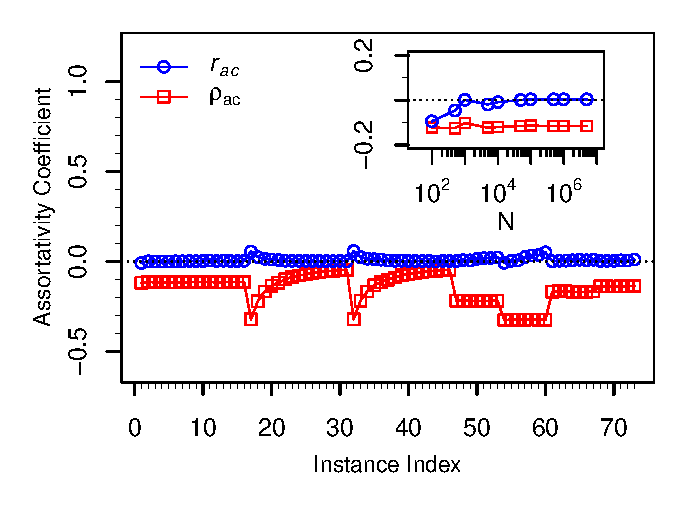
\includegraphics[width=0.6\columnwidth]{figs/ba-ac}
    \caption{Please write your figure caption here}
    \label{fig:ba-ac}       % Give a unique label
\end{figure}

In section \ref{sec:2.2}, we've discussed two methods to measure the network assortativity. Fig\cite{fig:1} Two measurements of assortativity coefficient .  We generate 79 BA networks with different parameters: $N$, number of the vertices; $m_0$, number of start vertices and $\Delta m$, number of edges to be added each timestep. We can get two observations  from the inner smaller figure. One is that When $N$ increasing dramatically, the Spearman measurement keeps stable, while the Pearson measurement reaches to 0. Another observation is that the magnitude of the Spearman result is much bigger than the Pearson one, especially when $N$ is large. The outer figure strengthen these two observations suggesting that the Spearman measurement is more stable and sensitive to the Spearman measurement.

\subsection{centrality correlations}

\begin{figure}
    \centering
    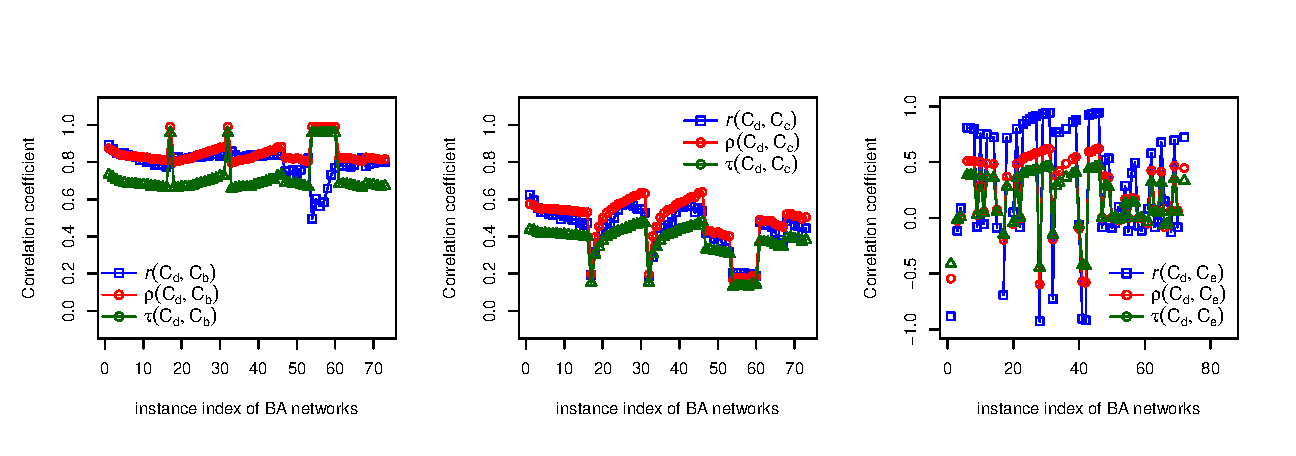
\includegraphics[width=0.96\columnwidth]{figs/ba-correlations}
    \caption{Three correlation in BA networks}
    \label{fig:2}       % Give a unique label
\end{figure}

Fig \ref{fig:2} shows the results of three correlations in BA networks. Regarding to all three measurements, degree and betweenness has a high correlation (greater than 0.6 for most cases), degree and closeness has a middle correlation (around 0.5), degree and eigenvector correlation varies much (from -0.9 to 0.9). The rank correlation $\rho$ and $\tau$ have the same trend in all cases, but $\rho$ is always higher then $\tau$. For correlations $(D_c, B_c)$, when $\Delta m=1$, the rank correlation $\rho$ and $\tau$ is much higher than $r$.

\subsection{relation between network properties and correlations}
As described in Sec \ref{sec:2}, the computation of network properties, such as average shortest path, cluster coefficient and degree assortativity are much easier then the computation of centrality metrics like betweenness and eigenvector. More over, the scatter plot (fig \ref{fig:ba-scatter}) suggests that their exists a relationship between the network properties and centrality correlations. Hence, we try to find out which network property has the most influence on a certain centrality correlation (\eg Spearman correlation between degree and betweenness $\rho(D,B)$). Here we use the multivariate linear regression model to investigate this relationship.











\section{Centrality rank correlation in real networks}
\label{sec:rn}
In \cite{newman2003mixing}, Newman adopted a loose classification that divided real networks into three categories: social, technological and biological. In \cite{Nej2003The}, he added a new category, information networks, consisting knowledge networks like citation network and World Wide Web (WWW) network. Here we take former classification, and classify the citation network to social networks, the WWW network to technological network.
\subsection{Data Set}
\label{sec:rn-datasets}
Thanks to the Internet, we have a chance to get rich network datasets from former researchers. The dataset in this paper are downloaded from four site: personal site of Newman, SNAP, Pajek and CCNR (see footnote of table \ref{tab:rn-description} for download URLs). We know that network could be divided as undirected and directed. The interpretation and computation of network centrality between undirected and directed are a little different. To make it simple and comparable, we treat all of our networks as undirected.    To help readers understand the classification and keep the description table \ref{tab:rn-description}, we will give explanations of many types of networks.
\subsubsection{Social networks}
A social network is a social structure made up of a set of people or groups of people as vertices and interactions between them as edges. In social language, vertices are often called social actors and edges are called social ties. The interactions could be friendship between individual, business relationship between companies, sex relationship and \etc. In early researches, sampled datasets are collected by questionnaire or interviews. Such methods are labor-intensive and therefor only limited size of network can be observed. Thanks to the rise of Internet, today we could get millions of records from the online social networks. According to the sample and construct methods, these social networks of our datasets could be divided into more specified types:
\setlist[description]{font=\bfseries}
\begin{description}[leftmargin=0cm]
\item [ego network] Ego networks consist of a focal node (``ego") and the nodes to whom ego is directly connected to (these are called "alters") plus the ties, if any, among the alters. In Facebook like  networks, these alters are friends lists of a center ego, so they are also called social circles. In our datasets, these named with ``ego-" are ego networks. Note that we use combined egonets instead of a single egonet. For example, the ``ego-facebook" is combined by 10 single ego networks.
\item [whole network] When merging all ego networks together, we could get a whole network. Often it's not very difficult for online social network providers to construct a whole network, since they have all the related records of the network. However, its not a easy work to construct a whole network by digging the social sites. In our datasets, these named with ``soc-'' are whole networks.
\item [email network] Email network is also a kind of communication network: given a set of email messages, each node corresponds to an email address, each edge between node $i$ and $j$ represents that there exists at least one message communication between $i$ and $j$.
\item [co-author network] Co-author networks are also called scientists collaboration networks: nodes represent scientist, edges represent collaborations. If an author $i$ co-authored a paper with author $j$, then there exists an edge between $i$ and $j$. In our datasets, these named with ``ca-'' are coauthor networks.
\item [co-citation network] Like co-author networks, in co-citation networks nodes represent papers and edges represent citations.  If a paper $i$ cites paper $j$, the graph contains a edge between $i$ to $j$. In our datasets, these named with ``cit-` are citation networks.
\item [co-purchasing network] In co-purchasing network, nodes represent products and edges represent co-purchasing: if a product $i$ is frequently co-purchased with product $j$, then there exist an edge between $i$ and $j$.
\item [co-actor network] In co-actor network, nodes represent actor and edges represent co-actor: if a actor $i$ co-actor with actor $j$ in a movie, then there exists an edge between $i$ and $j$.
\end{description}

\subsubsection{Technological networks}
Technological networks are man-made networks which are designed typically for distribution of some commodity or resource, such as electricity or information. In our datasets, these man-made networks are:
\setlist[description]{font=\bfseries}
\begin{description}[leftmargin=0cm]
\item [Power grid] The electric power grid is a network of high-voltage three-phase transmission lines that spans a country or a portion of a country(as opposed to the local low-voltage a.c. power delivery lines that span individual neighborhoods). An undirected, unweighted network representing the topology of the Western States Power Grid of the United States.
\item [Airlines] Airlines network is one of many transportation networks. The nodes represent airports and edges represent flight lines.
\item [Autonomous System networks] The routers that route package from one network to another are one of the most important components of Internet infrastructure. Autonomous System is a collection of connected IP routing prefixes, typically controlled by Internet Service Provider (ISP). To construct a view global Internet routing system, we often focus on the AS-level routers that exchange packages among different ASes. University of Oregon Route Views Project and The Center for Applied Internet Data Analysis (CAIDA) provide tools to probe the Internet to analyze topology and performance. The underlying techniques of these tools are BGP route logs and traceroute utility.
\item [Peer-to-peer networks] P2P file sharing allows users to access media files such as books, music, movies, and games using a P2P software program that searches for other connected computers on a P2P network to locate the desired content. In p2p network, nodes represent hosts and edges represent connections between the hosts. In our datasets, a sequence of snapshots of the Gnutella peer-to-peer file sharing network were collected and they are named with ``p2p-''.
\item [Web networks] In web networks, nodes represent webpages and edges are hyperlinks between them. Since the number of webpages in the Internet is too huge to build the whole network, we usually take webpages in specified domains as a sample, e.g. the data collection``web-ND'' represents webpage connection in University of Notre Dame (with domain nd.edu). Another construction method is through search engine query, e.g. the data collection ``web-qry-ca'' is constructed by expanding a 200-page response set to a search engine query 'California'.
\item [terror news network] The Reuters terror news network is based on all stories released during 66 consecutive days by the news agency Reuters concerning the September 11 attack on the U.S., beginning at 9:00 AM EST 9/11/01. The vertices of a network are words (terms); there is an edge between two words if they appear in the same text unit (sentence).
\item [dictionary network] In dictionary network, vertices represent terms and edges represent paraphrasing relations: if a term $i$ is used to describe the meaning of term $j$, then there exists an edge between them. In our datasets, ``foldoc'' is a searchable dictionary containing over 13000 definitions of terms.
\end{description}

\subsubsection{Biological networks}
Many biological systems could be usefully represented as networks, e.g. neural networks, protein interaction networks and metabolic networks. \textbf{Neural networks} try to represent the topology of real neural networks, that is how individual neurons are connected. \textbf{Protein interaction networks} describe the mechanistic physical interactions between proteins. Opposed to the physical interaction among proteins, \textbf{metabolic networks} consider the chemical reactions among metabolites: vertices represent metabolic substrates, edges represent known metabolic reaction between the substrates.

\subsection{Results and analysis}
The results of real networks are showed in table \ref{rn-r}. We take the similar strategies to analyze. However, we find that


\subsubsection{network properties}
Network properties of real networks are much more complicate then model ones. There is no simple links between them. 

For assortativity coefficient, network types play an important role. Most of social networks has positive coefficient, which implies homogeneity of social behaviors: famous person always have direct connect with famous person, while normal person own more normal person friends. On the contrary, technological networks shows a negative coefficient, which compatible with phenomenon in technology world: local router (low degree)  will be connected with upper level router (high degree) instead of other local router. For biological networks, their coefficient is rather small,  implying that they don't have this assortativity pattern.

We may also note that the trend of two assortativity computing methods is similar. The difference is that rank correlation method $\rho_{ac}$ is more sensitive, when coefficient trends to be positive, they are higher than $r_{ac}$, and vice versa. 
%
% For one-column wide figures use
\begin{figure}
    \centering
    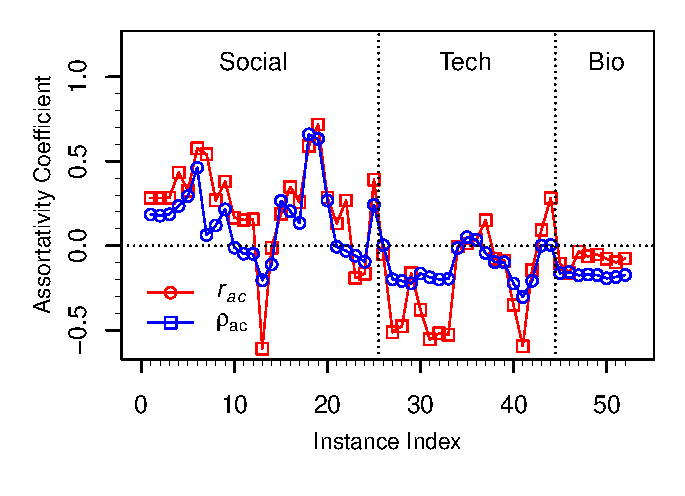
\includegraphics[width=0.6\columnwidth]{figs/rn-ac}
    \caption{Please write your figure caption here}
    \label{fig:rn-ac}       % Give a unique label
\end{figure}
\subsubsection{centrality correlations}


\begin{figure}
    \centering
    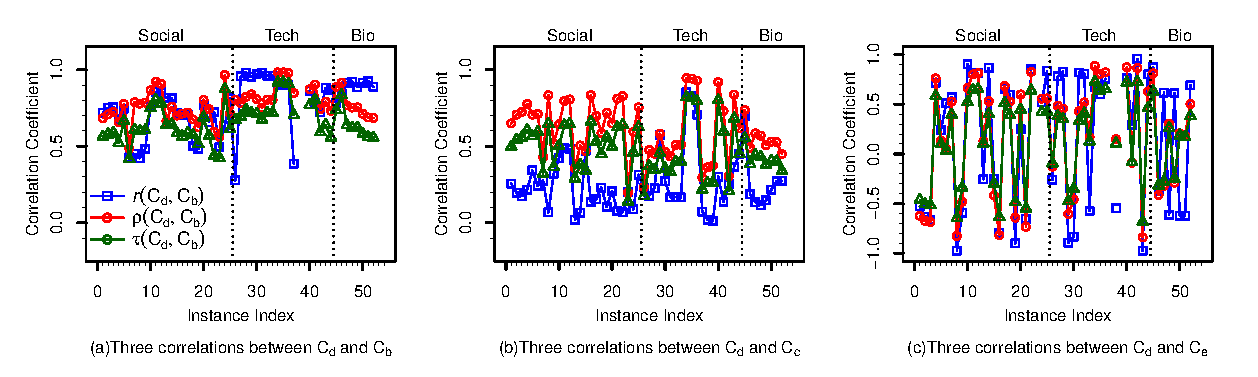
\includegraphics[width=0.96\columnwidth]{figs/rn-correlations}
    \caption{Rank correlation of real networks}
    \label{fig:rn-correlations}       % Give a unique label
\end{figure}

\subsubsection{relation between properties and correlations}

\section{Conclusion}

\section{References}
\bibliography{refs}

%
%appendix
\newpage

\appendixtitles{no} %Leave argument "no" if all appendix headings stay EMPTY (then no dot is printed after "Appendix A"). If the appendix sections contain a heading then change the argument to "yes".
\appendixsections{multiple} %Leave argument "multiple" if there are multiple sections. Then a counter is printed ("Appendix A"). If there is only one appendix section then change the argument to "one" and no counter is printed ("Appendix").
\appendix

The large datasets results are placed here in appendices: appendix \ref{app:ba} for BA networks and appendix \ref{app:rn} for real networks.

\section{BA networks}
\label{app:ba}
\setcounter{table}{0}
\renewcommand{\thetable}{A\arabic{table}}
\setcounter{figure}{0}
\renewcommand{\thefigure}{A\arabic{figure}}
In appendix \ref{app:ba}, there are 73 networks generated by BA model according to four types of patterns: increase of $N$, $m_0$, $\Delta m$ and $\Delta m=1$. We don't list all of them, just put 5 entries for each generation pattern. To save space, when list properties in table \ref{tab:ba-r} , we don't include all centrality correlations. Instead we select three correlation methods between degree and betweenness correlation (Kendall's $\tau(D_c,B_c)$, Pearson's $r(D_c,B_c)$ and Spearman's $\rho(D_c,B_c)$) as comparation. But we plot all of the correlations in figure \ref{fig:ba-correclation}.

%
% For tables use
\begin{table}[b]
\resizebox{0.96\textwidth}{!}{\begin{minipage}{\textwidth}
\caption[Text]{network properties and centrality correlations of BA model
\footnote{This table is the network properties and centrality correlations of 73 networks generated by BA model. Instance index Idx is listed according to the variation of three parameters in BA model:
increase of  $N$($N\uparrow $), increase of $\Delta m$($\Delta m\uparrow$), increase of $m_0$( $m_0\uparrow$) and a special case $\Delta m=1$.
}}
\label{tab:ba-r}       % Give a unique label
% For LaTeX tables use
\begin{tabular}{c c c c c  c c c c c  c c c c}
\hline\noalign{\smallskip}

 &Idx& $N$	& $m0$ & $\Delta m$ 	& $l$ & $C$ & $r_{ac}$ & $\rho_{ac}$ & $\tau(C_d, C_b)$ & $r(C_d, C_b)$ & $\rho(C_d, C_b)$ & $\rho(C_d, C_c)$  & $\rho(C_d, C_e)$\\
&	&$(e^{+4})$	&	&	&	&$(e^{-3})$	&	&	&	&	&	&	&	\\
\noalign{\smallskip}\hline\noalign{\smallskip}
\multirow{3}{*}{ $N \uparrow$}
&$1$	&	$1$	&	$5$	&	$5$	&	$3.72$	&	$4.98$	&	$-0.01$	&	$-0.12$	&	$0.73$	&	$0.89$	&	$0.87$	&	$0.58$	&	$-0.54$\\
&$2$	&	$2$	&	$5$	&	$5$	&	$3.95$	&	$2.76$	&	$0.00$	&	$-0.11$	&	$0.72$	&	$0.87$	&	$0.86$	&	$0.57$	&	$NA$\footnote{
Here NA means the value is unknown. This is caused by the failure of  $C_e$ computation.
}\\
&$3$	&	$3$	&	$5$	&	$5$	&	$4.06$	&	$1.99$	&	$0.00$	&	$-0.12$	&	$0.70$	&	$0.85$	&	$0.85$	&	$0.56$	&	$-0.03$\\
&$4$	&	$4$	&	$5$	&	$5$	&	$4.13$	&	$1.63$	&	$0.00$	&	$-0.11$	&	$0.69$	&	$0.84$	&	$0.84$	&	$0.55$	&	$0.01$\\
&$5$	&	$5$	&	$5$	&	$5$	&	$4.20$	&	$1.31$	&	$0.00$	&	$-0.12$	&	$0.69$	&	$0.85$	&	$0.84$	&	$0.55$	&	$NA$\\
\vdots  & \vdots \\
\multirow{5}{*}{ $\Delta m \uparrow$}
&$17$	&	$10$	&	$17$	&	$1$	&	$10.82$	&	$3.59$	&	$0.06$	&	$-0.32$	&	$0.96$	&	$0.80$	&	$0.99$	&	$0.20$	&	$-0.19$\\
&$18$	&	$10$	&	$17$	&	$2$	&	$6.09$	&	$1.28$	&	$0.03$	&	$-0.22$	&	$0.66$	&	$0.82$	&	$0.80$	&	$0.40$	&	$0.37$\\
&$19$	&	$10$	&	$17$	&	$3$	&	$5.15$	&	$0.97$	&	$0.01$	&	$-0.17$	&	$0.66$	&	$0.83$	&	$0.80$	&	$0.45$	&	$NA$\\
&$20$	&	$10$	&	$17$	&	$4$	&	$4.68$	&	$0.98$	&	$0.01$	&	$-0.13$	&	$0.67$	&	$0.82$	&	$0.81$	&	$0.50$	&	$-0.06$\\
&$21$	&	$10$	&	$17$	&	$5$	&	$4.37$	&	$1.06$	&	$0.01$	&	$-0.12$	&	$0.67$	&	$0.82$	&	$0.81$	&	$0.53$	&	$0.49$\\
\vdots  & \vdots \\
\multirow{5}{*}{ $\Delta m=1$}
&$54$	&	$10$	&	$3$	&	$1$	&	$13.80$	&	$0.01$	&	$-0.01$	&	$-0.33$	&	$0.96$	&	$0.50$	&	$0.99$	&	$0.17$	&	$0.17$\\
&$55$	&	$10$	&	$5$	&	$1$	&	$12.88$	&	$0.07$	&	$0.00$	&	$-0.32$	&	$0.96$	&	$0.60$	&	$0.99$	&	$0.18$	&	$0.00$\\
&$56$	&	$10$	&	$7$	&	$1$	&	$12.95$	&	$0.26$	&	$0.01$	&	$-0.32$	&	$0.96$	&	$0.56$	&	$0.99$	&	$0.18$	&	$0.18$\\
&$57$	&	$10$	&	$9$	&	$1$	&	$12.51$	&	$0.59$	&	$0.02$	&	$-0.32$	&	$0.96$	&	$0.58$	&	$0.99$	&	$0.17$	&	$0.18$\\
&$58$	&	$10$	&	$11$	&	$1$	&	$12.42$	&	$1.10$	&	$0.03$	&	$-0.32$	&	$0.96$	&	$0.66$	&	$0.99$	&	$0.17$	&	$0.00$\\
\vdots  & \vdots \\
\multirow{5}{*}{ $m_0 \uparrow$}
&$69$	&	$10$	&	$7$	&	$4$	&	$4.75$	&	$0.57$	&	$0.00$	&	$-0.14$	&	$0.68$	&	$0.79$	&	$0.82$	&	$0.52$	&	$0.47$\\
&$70$	&	$10$	&	$9$	&	$4$	&	$4.72$	&	$0.64$	&	$0.00$	&	$-0.14$	&	$0.68$	&	$0.79$	&	$0.82$	&	$0.51$	&	$0.07$\\
&$71$	&	$10$	&	$11$	&	$4$	&	$4.71$	&	$0.72$	&	$0.01$	&	$-0.14$	&	$0.67$	&	$0.81$	&	$0.82$	&	$0.51$	&	$NA$\\
&$72$	&	$10$	&	$13$	&	$4$	&	$4.68$	&	$0.80$	&	$0.01$	&	$-0.14$	&	$0.67$	&	$0.80$	&	$0.81$	&	$0.50$	&	$0.45$\\
&$73$	&	$10$	&	$15$	&	$4$	&	$4.71$	&	$0.87$	&	$0.01$	&	$-0.14$	&	$0.67$	&	$0.80$	&	$0.82$	&	$0.50$	&	$NA$\\
\noalign{\smallskip}\hline
\end{tabular}
\end{minipage} }
\end{table}
%

\section{Real networks}
\label{app:rn}
\setcounter{table}{0}
\renewcommand{\thetable}{B\arabic{table}}
\setcounter{figure}{0}
\renewcommand{\thefigure}{B\arabic{figure}}
In appendix \ref{app:rn}, there are 52 networks generated from real network dataset collections. We class these dataset collections into 3 loose categories: social, technological and biological. Table \ref{tab:rn-description} give a concise description of real networks datasets, you can see section{sec:rn-description} for a more comprehensive understanding. Table{tab:rn-r} shows the calculation results of real networks, we have 9 centrality correlations: 3 correlation methods combined with 3 centrality pairs. To make the table tight so that we can list them all, we use $(D,B)$ represents centrality correlation between degree and betweenness, which was noted as $(C_D,C_B)$ before, and $(D,C)$ for $(C_D,C_C)$, $(D,E)$ for $(C_D,C_E)$.

In table \ref{tab:ba-r} and \ref{tab:rn-r}, you may notice the `NA' values, most of them are related to eigenvector centrality($C_e$ or $E$) correlations. These NAs is called by the failure of eigenvector calculation. In eigenvector calculation, power iteration is commonly used algorithm. R program also take this algorithm, and the default maximum number of iteration is 1000. If R are running to the maximum iteration, but still not to get to the convergence, an error occurs. In this case, we treat the eigenvector as `NA', an unknown value. Therefor the following correlation calculation related to eigenvector is also set to be `NA'.

%
% For tables use
\begin{table*}[t]
\resizebox{0.96\textwidth}{!}{\begin{minipage}{\textwidth}
\caption[Text]{Description of real networks
\footnote{Idx: index number, used in later analysis; Source: sites to find these collections; $|V|$: number of vertices; $|E|$: number of edges. Please refer section \ref{sec:rn-datasets} for more comprehensive description or go to the following download sites.
}}
\label{tab:rn-description}       % Give a unique label
\newcounter{magicrownumbers}
\newcommand\rownumber{\stepcounter{magicrownumbers}\arabic{magicrownumbers}}
\begin{tabular}{L{0.1cm} l  L{2.4cm}   L{1.4cm}   l l   L{9.5cm}}
\toprule\noalign{\smallskip}
% header
	&	Idx	&	Name	&	Source	&	$|V|$	&	$|E|$	&	Description	\\
%
%hline with small skip
\noalign{\smallskip}\midrule\noalign{\smallskip}
% social networks
\parbox[t]{1mm}{\multirow{20}{*}{\rotatebox[origin=c]{90}{Social}}}
	&\rownumber & ca-CondMat-99		&	\multirow{6}{\linewidth}{Newman\footnote{Newman's personal site dataset collections: \url{http://www-personal.umich.edu/~mejn/netdata/}} \cite{newman2001structure, newman2006finding}	  }	 &	$16726$		&	$47594$		& \multirow{6}{\linewidth}{\textbf{Coauthor networks}, constructed from the e-print arXiv archive(\url{www.arxiv.org}) on Condensed Matter, Astrophysics and High-Energy Theory.  The file tail indicates the year of the data collection. The last one is a coauthor network of scientists working on network theory and experiment. }	\\
	&\rownumber & ca-CondMat-03		&	&	$31163$		&	$120029$		&	\\
	&\rownumber & ca-CondMat-05		&	&	$40421$		&	$175692$		&   \\
	&\rownumber & ca-AstroPh-99		&	&	$16706$		&	$121251$		&	\\
	&\rownumber & ca-HepTh-99			&	&	$8361$			&	$15751$		&  	\\
	&\rownumber & ca-netscience-06	&	&	$1589$			&	$2742$			& 	\\
	\cmidrule{3-7}
	&\rownumber &ego-Facebook	&\multirow{17}{\linewidth}{SNAP\footnote{Stanford Large Network Dataset Collection: \url{http://snap.stanford.edu/data/index.html}}  \cite{leskovec2012learning, yang2015defining, leskovec2007graph, leskovec2005graphs}	 }	& $4,039$ 	& $88,234$ &
	\multirow{3}{\linewidth}{\textbf{Combined Ego networks}, sampled from large online social networks Facebook, Google+ and Twitter}	\\
	&\rownumber &ego-Gplus		&		& $107614$ 	& $13673453$ &\\
	&\rownumber &ego-Twitter		&		& $81306$ 	& $1768149$ &\\
	&\rownumber &soc-Epinions1	&		& $75879$ 	& $508837$ &
	\multirow{3}{\linewidth}{sampled from online social networks Epionions and Slash}	\\
	&\rownumber &soc-Slash0811	&		& $77360$ 	& $905468$ &\\
	&\rownumber &soc-Slash0922	&		& $82168$ 	& $948464$ & \\
	&\rownumber &email-EuAll	&		& $265214$ 	& $420045$ & \multirow{2}{\linewidth}{\textbf{Email networks}}\\
	&\rownumber &email-Enron	&	& $36692$ 	& $183831$ &  \\
	&\rownumber &ca-DBLP	&		& $317080$ 	& $1049866$ &\multirow{6}{\linewidth}{\textbf{Co-author networks}, constructed from DBLP community and e-print arXiv archive}\\
	&\rownumber &ca-AstroPh	&	& $18772$ 	& $198110$ & \\
	&\rownumber &ca-CondMat	&	& $23133$ 	& $93497$ & \\
	&\rownumber &ca-GrQc	&			& $5242$ 	& $14496$ &\\
	&\rownumber &ca-HepPh&		& $12008$ 	& $118521$ &\\
	&\rownumber &ca-HepTh&	& $9877$ 	& $25998$ & \\
	\cmidrule{3-7}
	&\rownumber & actors	&\multirow{2}{\linewidth}{Pajek\footnote{Pajek  dataset collections: \url{http://vlado.fmf.uni-lj.si/pub/networks/data/default.htm}}\cite{barabasi1999emergence, jonescomputational}}	& $520223$   &$1470418$ 	&\textbf{Co-actors networks}, based on www.imdb.com\\
	&\rownumber & ca-Geom  	&	& $7343$   &$11898$ 	&\textbf{Co-author network} in Computational Geometry.\\
%
% hline with small skip
\noalign{\smallskip}\midrule\noalign{\smallskip}
%
% Information networks
\parbox[t]{1mm}{\multirow{10}{*}{\rotatebox[origin=c]{90}{Informational}}}
	&\rownumber &cit-HepPh	&\multirow{4}{\linewidth}{SNAP  \cite{leskovec2005graphs, gehrke2003overview, leskovec2007dynamics}	 }	& $34546$ 	& $421578$ &  \multirow{2}{\linewidth}{\textbf{Co-citation networks} from the e-print arXiv archive}\\
	&\rownumber &cit-HepTh	&	& $27770$ 	& $352807$ & \\
	&\rownumber &com-Amazon	&	& $334863$ 	& $925872$ & \textbf{Co-purchasing network} of the Amazon website.\\
	\cmidrule{3-7}
	&\rownumber &web-NotreDame	&\multirow{8}{\linewidth}{Pajek \cite{albert1999internet, corman2002studying, langville2006reordering, kamvar2003exploiting}}&	 $325729$			&	$1497134$	&\multirow{5}{\linewidth}{\textbf{World Wide Web networks} for domains at Notre Dome, Stanford and Berkeley-Stanford, and for search engine queries like `California' and `epa' }\\
	&\rownumber &web-Stanford		&				&	$281903$				& 	$2312497$		&\\
	&\rownumber &web-BerkStan		&				&	$685230$				&	$7600595$		& \\
	&\rownumber &web-qry-ca			&				&	$9664$					&	$15969$		&\\
	&\rownumber &web-query-epa		&				&	$4772$					&	$8909$			& \\
	&\rownumber &terror news	&		&	$13314$				&	$243447$		& \textbf{Reuters terror news network}\\
	&\rownumber &foldoc				&				&	$13356$				&	$120238$		& FOLDOC \textbf{dictionary network}.\\
%
% hline with small skip 
\noalign{\smallskip}\midrule\noalign{\smallskip}
%
% technology networks
\parbox[t]{1mm}{\multirow{16}{*}{\rotatebox[origin=c]{90}{Technological}}}
	&\rownumber &power grid	&Newman	&	$4941$			&	$6594$		& \textbf{Power grid network}, data citation \cite{watts1998collective}\\
	\cmidrule{3-7}
	&\rownumber &as-060722			&\multirow{7}{\linewidth}{SNAP\cite{leskovec2005graphs, ripeanu2002mapping}} 						&	$22963$				&	$48436$	&\multirow{5}{\linewidth}{\textbf{Internet AS networks}, constructed by BGP (Border Gateway Protocol) logs from University of Oregon Route View Project. }\\
	&\rownumber &as-980101			& 		&	$3213$				& $11710$		&\\
	&\rownumber &as-990101			& 				&		$531$				&	$2527$	&\\
	&\rownumber &as-000101			& 				&		$3570$				&	$14783$	&\\
	&\rownumber &as-010331			& 				&		$10670$			&	$22003$	&\\
	&\rownumber &as-Caida-1015   		&		 		&		$26258$			&	$107202$	& \multirow{2}{\linewidth}{\textbf{Internet AS relationship networks}, constructed by BGP logs and relationship inference algorithms, see  \href{ http://www.caida.org/data/as-relationships/}{caida}  }\\
	&\rownumber &as-Caida-1105   		&				&		$26475$			&	$106762$	& \\
	&\rownumber &p2p-Gnutella04   		&				&		$10876$			&	$39994$	&  \multirow{3}{\linewidth}{\textbf{p2p networks}, Gnutella peer-to-peer file sharing networks}\\
	&\rownumber &p2p-Gnutella06   		&				&		$8717$				&	$31525$	& \\
	&\rownumber &p2p-Gnutella08		&				&		$6301$				&	$20777$	& \\
	\cmidrule{3-7}
	&\rownumber &US air lines			&Pajek				&	$332$					&	$2126$			& US air lines\\
%
% hline
\noalign{\smallskip}\midrule\noalign{\smallskip}
% Biological
\parbox[t]{1mm}{\multirow{8}{*}{\rotatebox[origin=c]{90}{Biological}}}
	&\rownumber &neural network &Newman		&	$297$			&	$2151$		&	\textbf{Neural network} of C. Elegans, data citation \cite{watts1998collective}\\
	\cmidrule{3-7}
	&\rownumber &protein-protein  &\multirow{7}{\linewidth}{CCNR\footnote{CCNR dateset collections:\url{http://www3.nd.edu/~networks/resources.htm}}\cite{watts1998collective, jeong2001lethality, jeong2000large}}		&	$1870$		&	$4480$		&\textbf{Protein interaction network} data (for yeast).\\
	&\rownumber &celluar-AA			&			&	$1485$	& 	$3400$		& \multirow{6}{\linewidth}{\textbf{Cellular networks} and its \textbf{metabolic networks}, the file tail indicates different organisms.}\\
	&\rownumber &celluar-AB			&			& $1416$		& 	$3230$		&\\
	&\rownumber &celluar-AG			&			& $1567$		& 	$3631$		&\\
	&\rownumber &metabolic-AA			&			& $1057$		& 	$2527$		&\\
	&\rownumber &metabolic-AB			&			& $993$		& 	$2368$		&\\
	&\rownumber &metabolic-AG			&			& $1268$		& 	$3011$		&\\
% bottom hline
\noalign{\smallskip}\bottomrule
\end{tabular}
\end{minipage} }
\end{table*}
%
%
% real network result tables
\begin{table*}
\resizebox{0.92\textwidth}{!}{\begin{minipage}{\textwidth}
\caption[Text]{Network properties of real networks
\footnote{This table shows network properties and centrality correlations of real networks. Idx: index number, same as table \ref{tab:rn-description}; $l$: average path length; $C$: cluster coefficient; $r_{ac}$ and $\rho_{ac}$: degree assotativity. We use $r$, $\rho$ and $\tau$ to represent Pearson, Spearman and Kendall correlation methods, and $D$, $B$, $C$ and $E$ to represent degree, betweenness, closeness and eigenvector centrality metrics, therefore $r(D,B)$ represents the Pearson correlation coefficient between degree and betweenness centrality. Please see table \ref{tab:rn-description} for the description of datasets and section \ref{sec:rn-analysis} for the analysis of results. 
}}
\label{tab:rn-r}       % Give a unique label
\setcounter{magicrownumbers}{0}
\newcommand\rownumber{\stepcounter{magicrownumbers}\arabic{magicrownumbers}}

\begin{tabular}{L{0.25cm} l l l l   l l l l l   l l l l l}
\toprule\noalign{\smallskip}
    &   Idx &   $l$     &   $C$ &   $r_{ac}$    &   $\rho_{ac}$     &   $r(D,B)$    &   $r(D,C)$    &   $r(D,E)$    &   $\rho(D,B)$     &   $\rho(D,C)$     &   $\rho(D,E)$ &   $\tau(D,B)$     &   $\tau(D,C)$     &   $\tau(D,E)$\\
\noalign{\smallskip}\midrule\noalign{\smallskip}
\parbox[t]{1mm}{\multirow{25}{*}{\rotatebox[origin=c]{90}{Social}}}
    &   \rownumber    &   $6.63$	&	$0.36$	&	$0.18$	&	$0.28$	&	$0.72$	&	$0.26$	&	$-0.53$	&	$0.56$	&	$0.50$	&	$-0.46$	&	$0.68$	&	$0.65$	&	$-0.62$\\
    &   \rownumber    &   $5.77$	&	$0.28$	&	$0.18$	&	$0.28$	&	$0.75$	&	$0.20$	&	$-0.63$	&	$0.58$	&	$0.54$	&	$-0.50$	&	$0.71$	&	$0.71$	&	$-0.67$\\
    &   \rownumber    &   $5.50$	&	$0.25$	&	$0.19$	&	$0.28$	&	$0.76$	&	$0.17$	&	$-0.66$	&	$0.59$	&	$0.56$	&	$-0.51$	&	$0.72$	&	$0.72$	&	$-0.69$\\
    &   \rownumber    &   $4.80$	&	$0.43$	&	$0.24$	&	$0.43$	&	$0.68$	&	$0.22$	&	$0.72$	&	$0.52$	&	$0.61$	&	$0.58$	&	$0.66$	&	$0.78$	&	$0.76$\\
    &   \rownumber    &   $7.03$	&	$0.33$	&	$0.29$	&	$0.32$	&	$0.75$	&	$0.34$	&	$0.24$	&	$0.67$	&	$0.57$	&	$0.10$	&	$0.78$	&	$0.71$	&	$0.13$\\
    &   \rownumber    &   $5.82$	&	$0.69$	&	$0.46$	&	$0.58$	&	$0.43$	&	$0.24$	&	$0.51$	&	$0.42$	&	$0.60$	&	$0.04$	&	$0.48$	&	$0.71$	&	$0.05$\\
    &   \rownumber    &   $3.69$	&	$0.52$	&	$0.06$	&	$0.54$	&	$0.45$	&	$0.27$	&	$0.57$	&	$0.61$	&	$0.32$	&	$0.39$	&	$0.79$	&	$0.43$	&	$0.53$\\
    &   \rownumber    &   $2.86$	&	$0.22$	&	$0.12$	&	$0.27$	&	$0.42$	&	$0.07$	&	$-0.97$	&	$0.60$	&	$0.65$	&	$-0.65$	&	$0.78$	&	$0.83$	&	$-0.83$\\
    &   \rownumber    &   $3.89$	&	$0.17$	&	$0.22$	&	$0.38$	&	$0.48$	&	$0.32$	&	$-0.59$	&	$0.60$	&	$0.36$	&	$-0.34$	&	$0.79$	&	$0.52$	&	$-0.48$\\
    &   \rownumber    &   $4.31$	&	$0.07$	&	$-0.01$	&	$0.17$	&	$0.76$	&	$0.42$	&	$0.90$	&	$0.75$	&	$0.50$	&	$0.52$	&	$0.87$	&	$0.64$	&	$0.66$\\
    &   \rownumber    &   $4.02$	&	$0.02$	&	$-0.05$	&	$0.15$	&	$0.86$	&	$0.49$	&	$0.81$	&	$0.80$	&	$0.64$	&	$0.64$	&	$0.92$	&	$0.80$	&	$0.80$\\
    &   \rownumber    &   $4.07$	&	$0.02$	&	$-0.05$	&	$0.16$	&	$0.85$	&	$0.48$	&	$0.81$	&	$0.78$	&	$0.65$	&	$0.65$	&	$0.91$	&	$0.81$	&	$0.81$\\
    &   \rownumber    &   $4.12$	&	$0.00$	&	$-0.20$	&	$-0.61$	&	$0.82$	&	$0.02$	&	$-0.25$	&	$0.64$	&	$0.29$	&	$0.11$	&	$0.66$	&	$0.36$	&	$0.13$\\
    &   \rownumber    &   $4.03$	&	$0.09$	&	$-0.11$	&	$-0.01$	&	$0.82$	&	$0.07$	&	$0.87$	&	$0.64$	&	$0.38$	&	$0.40$	&	$0.76$	&	$0.51$	&	$0.53$\\
    &   \rownumber    &   $6.79$	&	$0.31$	&	$0.27$	&	$0.19$	&	$0.72$	&	$0.47$	&	$-0.25$	&	$0.59$	&	$0.34$	&	$-0.30$	&	$0.70$	&	$0.47$	&	$-0.42$\\
    &   \rownumber    &   $4.19$	&	$0.32$	&	$0.21$	&	$0.35$	&	$0.70$	&	$0.14$	&	$-0.79$	&	$0.56$	&	$0.66$	&	$-0.63$	&	$0.71$	&	$0.83$	&	$-0.82$\\
    &   \rownumber    &   $5.35$	&	$0.26$	&	$0.13$	&	$0.26$	&	$0.70$	&	$0.15$	&	$0.65$	&	$0.59$	&	$0.53$	&	$0.51$	&	$0.72$	&	$0.70$	&	$0.68$\\
    &   \rownumber    &   $6.05$	&	$0.63$	&	$0.66$	&	$0.59$	&	$0.50$	&	$0.23$	&	$0.59$	&	$0.57$	&	$0.45$	&	$0.39$	&	$0.68$	&	$0.59$	&	$0.53$\\
    &   \rownumber    &   $4.67$	&	$0.66$	&	$0.63$	&	$0.72$	&	$0.48$	&	$0.10$	&	$-0.90$	&	$0.51$	&	$0.56$	&	$-0.48$	&	$0.62$	&	$0.72$	&	$-0.64$\\
    &   \rownumber    &   $5.95$	&	$0.28$	&	$0.27$	&	$0.29$	&	$0.77$	&	$0.21$	&	$0.25$	&	$0.69$	&	$0.50$	&	$0.44$	&	$0.80$	&	$0.65$	&	$0.60$\\
    &   \rownumber    &   $7.17$	&	$0.00$	&	$-0.09$	&	$-0.17$	&	$0.64$	&	$0.09$	&	$0.52$	&	$0.87$	&	$0.46$	&	$0.42$	&	$0.97$	&	$0.59$	&	$0.56$\\
%hline
\noalign{\smallskip}\midrule\noalign{\smallskip}
%
% Information networks
\parbox[t]{1mm}{\multirow{10}{*}{\rotatebox[origin=c]{90}{Informational}}}
    &   \rownumber    &   $5.31$	&	$0.24$	&	$0.24$	&	$0.39$	&	$0.81$	&	$0.31$	&	$0.83$	&	$0.61$	&	$0.63$	&	$0.42$	&	$0.71$	&	$0.76$	&	$0.56$\\
    &   \rownumber    &   $4.33$	&	$0.15$	&	$-0.01$	&	$0.13$	&	$0.66$	&	$0.08$	&	$-0.65$	&	$0.57$	&	$0.62$	&	$-0.55$	&	$0.74$	&	$0.81$	&	$-0.73$\\
    &   \rownumber    &   $4.28$	&	$0.12$	&	$-0.03$	&	$0.27$	&	$0.72$	&	$0.07$	&	$0.85$	&	$0.44$	&	$0.64$	&	$0.64$	&	$0.60$	&	$0.83$	&	$0.82$\\
    &   \rownumber    &   $11.95$	&	$0.21$	&	$-0.06$	&	$-0.19$	&	$0.50$	&	$0.20$	&	$NA$	&	$0.42$	&	$0.14$	&	$NA$	&	$0.56$	&	$0.20$	&	$NA$\\
    &   \rownumber    &   $7.17$	&	$0.09$	&	$-0.05$	&	$-0.11$	&	$0.43$	&	$0.07$	&	$-0.52$	&	$0.73$	&	$0.23$	&	$-0.29$	&	$0.87$	&	$0.31$	&	$-0.38$\\
    &   \rownumber    &   $6.82$	&	$0.01$	&	$-0.11$	&	$-0.16$	&	$0.55$	&	$0.02$	&	$-0.55$	&	$0.25$	&	$0.33$	&	$0.14$	&	$0.34$	&	$0.45$	&	$0.18$\\
    &   \rownumber    &   $7.11$	&	$0.01$	&	$-0.11$	&	$-0.17$	&	$0.46$	&	$0.01$	&	$NA$	&	$0.21$	&	$0.33$	&	$NA$	&	$0.29$	&	$0.46$	&	$NA$\\
    &   \rownumber    &   $5.03$	&	$0.02$	&	$-0.22$	&	$-0.35$	&	$0.86$	&	$0.30$	&	$0.76$	&	$0.77$	&	$0.80$	&	$0.72$	&	$0.87$	&	$0.92$	&	$0.87$\\
    &   \rownumber    &   $4.50$	&	$0.01$	&	$-0.30$	&	$-0.59$	&	$0.78$	&	$0.14$	&	$0.29$	&	$0.80$	&	$0.60$	&	$-0.08$	&	$0.90$	&	$0.73$	&	$-0.09$\\
%hline
\noalign{\smallskip}\midrule\noalign{\smallskip}
%
% technology networks
\parbox[t]{1mm}{\multirow{16}{*}{\rotatebox[origin=c]{90}{Technological}}}
    &   \rownumber    &   $3.12$	&	$0.11$	&	$0.00$	&	$0.09$	&	$0.88$	&	$0.36$	&	$-0.97$	&	$0.64$	&	$0.68$	&	$-0.68$	&	$0.79$	&	$0.84$	&	$-0.84$\\
    &   \rownumber    &   $3.87$	&	$0.11$	&	$0.00$	&	$0.28$	&	$0.87$	&	$0.45$	&	$0.80$	&	$0.56$	&	$0.45$	&	$0.46$	&	$0.73$	&	$0.62$	&	$0.63$\\
    &   \rownumber    &   $18.99$	&	$0.10$	&	$0.00$	&	$-0.05$	&	$0.28$	&	$0.23$	&	$-0.26$	&	$0.67$	&	$0.18$	&	$-0.09$	&	$0.80$	&	$0.23$	&	$-0.13$\\
    &   \rownumber    &   $3.84$	&	$0.01$	&	$-0.20$	&	$-0.51$	&	$0.96$	&	$0.18$	&	$0.78$	&	$0.69$	&	$0.37$	&	$0.38$	&	$0.78$	&	$0.48$	&	$0.49$\\
    &   \rownumber    &   $3.77$	&	$0.01$	&	$-0.21$	&	$-0.48$	&	$0.98$	&	$0.23$	&	$0.83$	&	$0.74$	&	$0.35$	&	$0.35$	&	$0.82$	&	$0.45$	&	$0.46$\\
    &   \rownumber    &   $3.39$	&	$0.12$	&	$-0.22$	&	$-0.16$	&	$0.95$	&	$0.57$	&	$-0.89$	&	$0.72$	&	$0.46$	&	$-0.48$	&	$0.84$	&	$0.58$	&	$-0.60$\\
    &   \rownumber    &   $3.80$	&	$0.02$	&	$-0.16$	&	$-0.38$	&	$0.97$	&	$0.27$	&	$-0.83$	&	$0.71$	&	$0.36$	&	$-0.35$	&	$0.81$	&	$0.46$	&	$-0.46$\\
    &   \rownumber    &   $3.64$	&	$0.01$	&	$-0.19$	&	$-0.55$	&	$0.98$	&	$0.17$	&	$0.82$	&	$0.68$	&	$0.33$	&	$0.33$	&	$0.75$	&	$0.43$	&	$0.43$\\
    &   \rownumber    &   $3.86$	&	$0.01$	&	$-0.20$	&	$-0.52$	&	$0.96$	&	$0.17$	&	$0.81$	&	$0.72$	&	$0.40$	&	$0.41$	&	$0.80$	&	$0.51$	&	$0.52$\\
    &   \rownumber    &   $3.88$	&	$0.01$	&	$-0.19$	&	$-0.53$	&	$0.96$	&	$0.17$	&	$-0.57$	&	$0.72$	&	$0.40$	&	$0.13$	&	$0.80$	&	$0.51$	&	$0.17$\\
%
% hline
\noalign{\smallskip}\midrule\noalign{\smallskip}
%
% Biological
\parbox[t]{1mm}{\multirow{8}{*}{\rotatebox[origin=c]{90}{Biological}}}
    &   \rownumber    &   $4.64$	&	$0.01$	&	$-0.01$	&	$0.00$	&	$0.90$	&	$0.85$	&	$0.68$	&	$0.92$	&	$0.82$	&	$0.73$	&	$0.98$	&	$0.95$	&	$0.88$\\
    &   \rownumber    &   $4.57$	&	$0.01$	&	$0.05$	&	$0.01$	&	$0.90$	&	$0.83$	&	$0.60$	&	$0.92$	&	$0.82$	&	$0.64$	&	$0.98$	&	$0.94$	&	$0.80$\\
    &   \rownumber    &   $4.64$	&	$0.02$	&	$0.04$	&	$0.03$	&	$0.90$	&	$0.71$	&	$0.76$	&	$0.91$	&	$0.80$	&	$0.65$	&	$0.98$	&	$0.93$	&	$0.82$\\
    &   \rownumber    &   $2.74$	&	$0.40$	&	$-0.21$	&	$-0.14$	&	$0.72$	&	$0.25$	&	$0.96$	&	$0.59$	&	$0.21$	&	$0.72$	&	$0.74$	&	$0.30$	&	$0.86$\\
    &   \rownumber    &   $2.46$	&	$0.18$	&	$-0.16$	&	$-0.11$	&	$0.78$	&	$0.70$	&	$0.87$	&	$0.74$	&	$0.55$	&	$0.63$	&	$0.89$	&	$0.74$	&	$0.81$\\
    &   \rownumber    &   $6.81$	&	$0.06$	&	$-0.16$	&	$-0.18$	&	$0.85$	&	$0.19$	&	$-0.35$	&	$0.83$	&	$0.40$	&	$-0.33$	&	$0.92$	&	$0.51$	&	$-0.42$\\
    &   \rownumber    &   $4.49$	&	$0.00$	&	$-0.19$	&	$-0.07$	&	$0.91$	&	$0.22$	&	$-0.62$	&	$0.59$	&	$0.41$	&	$0.19$	&	$0.71$	&	$0.54$	&	$0.21$\\
    &   \rownumber    &   $4.40$	&	$0.00$	&	$-0.16$	&	$0.00$	&	$0.88$	&	$0.15$	&	$-0.62$	&	$0.72$	&	$0.49$	&	$0.18$	&	$0.84$	&	$0.63$	&	$0.20$\\
    &   \rownumber    &   $4.46$	&	$0.00$	&	$-0.19$	&	$-0.13$	&	$0.91$	&	$0.13$	&	$-0.65$	&	$0.57$	&	$0.41$	&	$-0.44$	&	$0.70$	&	$0.54$	&	$-0.57$\\
    &   \rownumber    &   $4.49$	&	$0.00$	&	$-0.19$	&	$-0.07$	&	$0.91$	&	$0.22$	&	$-0.62$	&	$0.59$	&	$0.41$	&	$0.19$	&	$0.71$	&	$0.54$	&	$0.21$\\
    &   \rownumber    &   $4.40$	&	$0.00$	&	$-0.16$	&	$0.00$	&	$0.88$	&	$0.15$	&	$-0.62$	&	$0.72$	&	$0.49$	&	$0.18$	&	$0.84$	&	$0.63$	&	$0.20$\\
    &   \rownumber    &   $4.46$	&	$0.00$	&	$-0.19$	&	$-0.13$	&	$0.91$	&	$0.13$	&	$-0.65$	&	$0.57$	&	$0.41$	&	$-0.44$	&	$0.70$	&	$0.54$	&	$-0.57$\\
% bottom hline
\noalign{\smallskip}\bottomrule
\end{tabular}
\end{minipage} }
\end{table*}
%




\end{document}

